\section{Action Path Models}
\label{ch:model}

In this chapter, we formalize few concepts and metrics in clickstream data,
and then describe a proposed clickstream model named \emph{Action Path model} 
based on recurrent nerual network that models a client side clickstream behavior. 
The action path is different than clickstream since 
a user may uses \emph{back button} or \emph{switch browser tabs} then jumps to visited web pages 
or parallel web pages, namely, a user performed a visit action.
A server side clickstream does not containing such detailed level of user clickstream. 
The term \emph{action path} is a generalized concept of clickstream, which replaces individual URLs 
to user actions (with backbutton and browser tab switch effects) in a browser. Figure \ref{fig:clickstream}
illustrates an simplified version of action path that compares vanilla clickstream.

\begin{figure}[H]
    \centering
    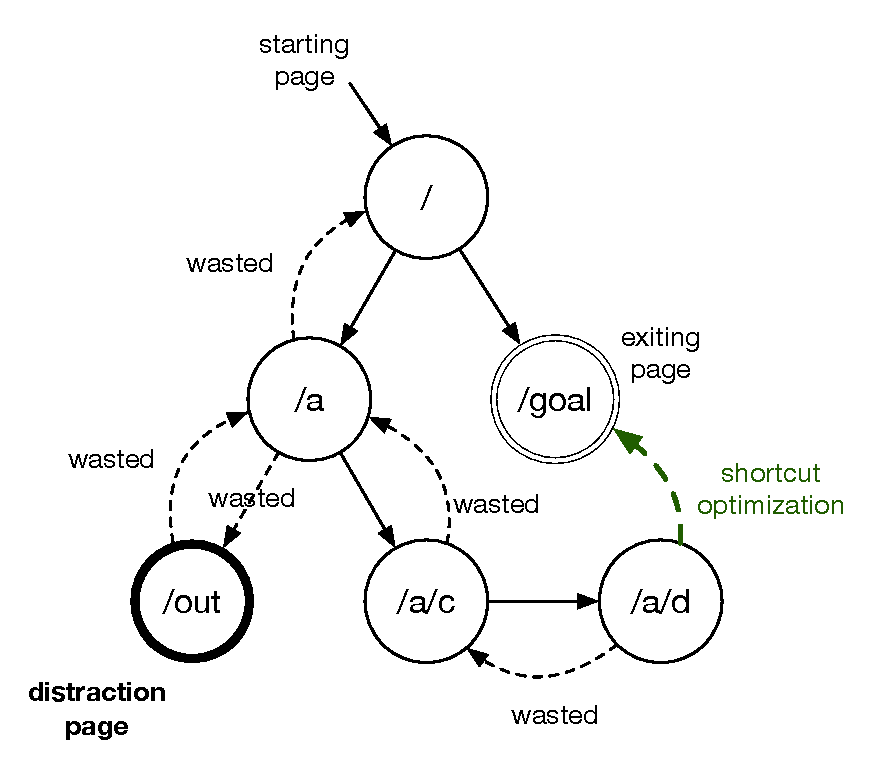
\includegraphics[width=0.5\textwidth]{figures/clickstream}
    \caption{A simple action path. A user starts from the starting page, and performed
    a series of page click actions, ends on a exiting page. 
    The server side records clickstream in the following order:
    / $\rightarrow$ /a $\rightarrow$ /out $\rightarrow$ /a/c $\rightarrow$ /a/d $\rightarrow$ /goal.
    However the actual user actions are: 
    / $\rightarrow$ /a $\rightarrow$ /out $\rightarrow$ /a $\rightarrow$ /a/c $\rightarrow$ /a/d 
    $\rightarrow$ /a/c $\rightarrow$ /a $\rightarrow$ / $\rightarrow$ /goal. 
    The records on server side lost interaction details between users and browsers.
    Node that /out is a distraction page in the graph, 
    which may located in a different website (e.g. advertisement), 
    and dashed arrorws are wasted user
    actions. The /goal page may not clear in the beginning of the clickstream, one can generate
    a shortcut optimization navigation to the /goal page while more clickstream context
    be presented, i.e. an optimized user actions is 
    / $\rightarrow$ /a $\rightarrow$ /a/c $\rightarrow$ /a/d $\rightarrow$ /goal.}
    \label{fig:clickstream}
\end{figure}

For a convinience of discussion, we indiscriminate the use of 
term \emph{action path} and \emph{clickstream} in
this chapter to indicate a series of user actions.

\subsection{Completion Effeciency}

An action path of a visiting session starts from a starting page and ends on a exiting page.
Since we consider the effect of browser back button and browser tab swtich, previous page could
easily be visited twice, if a user clicked the back button. Therefore, a page may directs
to multiple pages. \emph{For instance, an action path could degrade to a linked list if a user
click through to different pages without using back button and switching tabs; or an action
path could become a 1-to-n bipartite graph if a user use back button back to previous page
after clicked a page,} as shown in Figure \ref{fig:sim-action-path}.

As a result, we define the \emph{completion effeciency} based on shortest path from starting page
to exiting page, and stay duration of the action path. 

\begin{figure}[H]
    \centering

\begin{subfigure}[b]{0.55\textwidth}
    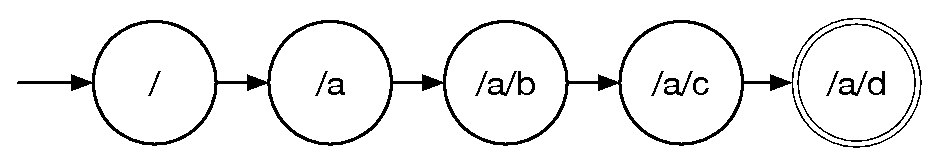
\includegraphics[width=1\textwidth]{figures/linked-list}
    \caption{}
    \label{fig:sim-action-1}
\end{subfigure}
    
\begin{subfigure}[b]{0.23\textwidth}
    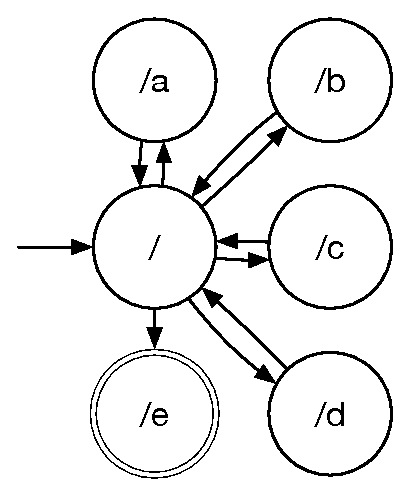
\includegraphics[width=1\textwidth]{figures/1ton}
    \caption{}
    \label{fig:sim-action-2}
\end{subfigure}

\caption{Two special case of an action path: linked list action path \ref{fig:sim-action-1}, and 
1-to-n bipartite graph action path \ref{fig:sim-action-2}.}
\label{fig:sim-action-path}
\end{figure}

Let an action path is represented on directed cyclic graph, each node represents a visited page,
and each edge has a weight that represents the stady duration of its tail node.
Assume the total stay duration of the shortest path from starting page to existing page
is $d_s$, and the total stay duration of the action path is $D$, 
the number of nodes in the shortest path is $n_s$, the total nodes 
in an action path is $N$, the \emph{completion effeciency $E$} is defined 
as follows Equation \ref{eqn:completion-effeciency}:

\begin{align}
\label{eqn:completion-effeciency}
\begin{split}
    E = w_1 \frac{n_s}{N} + w_2 \frac{d_s}{D}\\
    w_1 + w_2 = 1
\end{split}
\end{align}

where $w_1$, $w_2$ are hyperparameters to balancing the importance of action path 
and stay duration. According to the duscussion of two special case of action path,
it is easy to prove the range of $E$ is $(0, 1]$. As a complement, we define \emph{zero
completion efficiency} if and only if a user cannot complete a clickstream. Therefore
we have the range of $E$ is $[0, 1]$.

\paragraph{Remark 1} The definition of completion effeciency uses the term of shortest path,
which is the problem of finding a path between the starting page and exiting page
 in a action path (directed cyclic graph) such taht the sum of
the stay duration of its constitunent pages in minimized.
The problem can be solved by Dijkstra's shortest-path algorithm \cite{dijkstra1959note}.

\paragraph{Remark 2} An action path may increases with more nodes (pages) over time.
The starting page of an action path is always the first page when browser was opened.
However, one can always treat the current visited page is the exiting page due to we
do not know when an user will exit browsing over time. Consequently, $E$ is changing over
browsing.

\paragraph{Remark 3} We uses completion efficiency as a
feature for a classification task in Section \ref{sec:inter-general-feature}.

% TODO: 考虑是否还需要这个
% \subsection{Clickstream Overlap Ratio}

% Clickstreams can be overlapped one another, a simple overlapping can be formalized
% via a ratio of common pages and total pages in two clickstreams.
% Nevertheless the major concern of this method does not considering the completion effeciency
% of an action path. Completion effeciency seperates the importance of pages to two parts:
% pages distribute in the shortest path between starting page and exiting page, say Type-I page, 
% as well as pages do not distribute in the shortest path, say Type-II page.

\subsection{\emph{url2vec} Embedding}

The distributed representation of word2vec models achieve better performance 
in natural language processing,
Mikolov et al. \cite{DBLP:journals/corr/abs-1301-3781} introduced 
continous bag-of-word (CBOW) and skip-gram model as an efficient method for learning high-quality
vector representation of words, and CBOW is faster while skip-gram is slower but get better
performance for infrequent words. We convey similar idea from these models and propose our
\emph{url2vec} model for client side clickstream data.

The purpose of url2vec model is to construct URL representations to better predict 
the surrounding URLs in a clickstream. Briefly, given a clickstream of urls 
$\text{URL}_1, \text{URL}_2, ..., \text{URL}_T$, the objective of url2vec is to maximize the average
log softmax probability:

\begin{align}
\label{eqn:url2vecprob}
\begin{split}
    \frac{1}{T}\sum^{T}_{t=1}\sum_{-c \leq i \leq c, i \neq 0} {\log{p(\text{URL}_{t+i} | \text{URL}_t)}}\\
    p(\text{URL}_{t+i} | \text{URL}_t) = \frac{
        \exp{(v_{\text{URL}_{t+i}} ^\top v_{\text{URL}_t})}
    }{
        \sum_{\text{all URLs}} {\exp{(v_{\text{URL}_{t+i}} ^\top v_{\text{URL}_t})}}
    }
\end{split}
\end{align}

where $c$ is the size of embedding context, which is a function of starting page,
$v_{\text{URL}_t}$ is one-hot encoded representation of input URLs, and 
$v_{\text{URL}_{t+i}}$ is the vector embedding of output representations.

\paragraph{Remark 1} This model described by Equation \ref{eqn:url2vecprob} is essentially
a three layer neural network: input layer of \emph{one-hot} encoded URLs (a group of binaries
that a component of a one-hot encoded vector is a representative of a URL under a finite set
of existing URLs), a hidden layer of
feature representation and an output layer share weights to the learned embeddings of 
input URLs.

\paragraph{Remark 2} The probability in Equation \ref{eqn:url2vecprob} is impractical due to
$\nabla \log{p(\text{URL}_{t+i} | \text{URL}_t)}$ is large because of expnential items,
two numerical optimizations based on Hofmann Tree and Negative Sampling are proposed 
by Mikolv et al. \cite{mikolv2013embedding}.

\paragraph{Remark 3} The probability can also be interpret in Bayesian perspective,
which provides a intuition of this definition. $p(\text{URL}_{t+i} | \text{URL}_t)$
can be considered as a posterior probability. Since $v_{\text{URL}_t}$ was initialized
as an one-hot encoded vector input to the embedding neural network, the item can be treat
as a prior and the denominator is a normalization term.
Furthermore, the dot product between $v_{\text{URL}_{t+i}} ^\top$
and $v_{\text{URL}_t}$ is a representation of consine similarity, which represents
the closest surrounding URLs in same direction of vectors.

\subsection{Action Path Model}

Recurrent Neural Network (RNN) was describe by Werbos \cite{werbos1990rnn} and 
Rumelhart et al. \cite{Rumelhart:1988:LRB:65669.104451}, the original RNN 
generalize feedforward neural network for sequence based data.

Given a sequence of input $(i_1, i_2, ..., i_T)$, the original RNN computes a
sequence of outputs $(o_1, o_2, ..., o_T)$ 
by interating the activation function Equation \ref{eqn:bptt}:

\begin{align}
\label{eqn:bptt}
\begin{split}
    o_t = W_{oh} \sigma \left( W_{hi}i_{t} + W_{hh}i_{t-1}\right), t=1,2,...,T
\end{split}
\end{align}

where $\sigma(x) = \frac{1}{1+\exp\{-x\}}$,
and $W_{oh}, W_{hh}, W_{hi}$ are weight parameters between output, hidden and input layers.

The vanilla RNN transfers and maps a sequence to another sequence if and only if the inputs
and the outputs are aligned with equal length. Apparently, the major constrains of the vanilla RNN
is the model cannot address a problem if inputs and outputs provided in different length with 
complicated and non-monotonic relationships.

Stutskever et al. \cite{DBLP:journals/corr/SutskeverVL14} present a general end-to-end approach
to sequence learning model in machine translation that estimates the conditional probability of 
$p(o_1, o_2, ..., o_{T'} | i_1, i_2, ..., i_T)$ where $(i_1, i_2, ..., i_T)$ is an input sequence,
$(o_1, o_2, ..., o_{T'})$ is a corresponding output sequence, and $T$ is not required to be equal with $T'$.
Our model convey similar idea from it.

An \emph{action path} from user $i$ in session $j$ consist of 
a sequence of \emph{url2vec} embedded vectors $(U^{ij}_1, U^{ij}_2, ..., U^{ij}_n)$ 
and a sequence of time duration $(d^{ij}_1, d^{ij}_2, ..., d^{ij}_n)$, since each URL 
has a corresponding number that represents the time duration of a user spent on a given page.
Our action path model consist a context encoder and a context decoder. 

\subsubsection{Context Encoder}

Context encoder encodes URLs one by one and produces a context tensor that encodes 
the historical user actions, as shown in Figure \ref{fig:encoder}. 
In the encoder, we insert a starting mark ``<SOA>'' (\emph{Start of Action})
as a sign of start feeding URLs, and a trigger mark ``<COI>'' (\emph{Change of Intention}) as
a sign to trigger decoder to decodes encoded context tensor.

\begin{figure}[H]
    \centering
    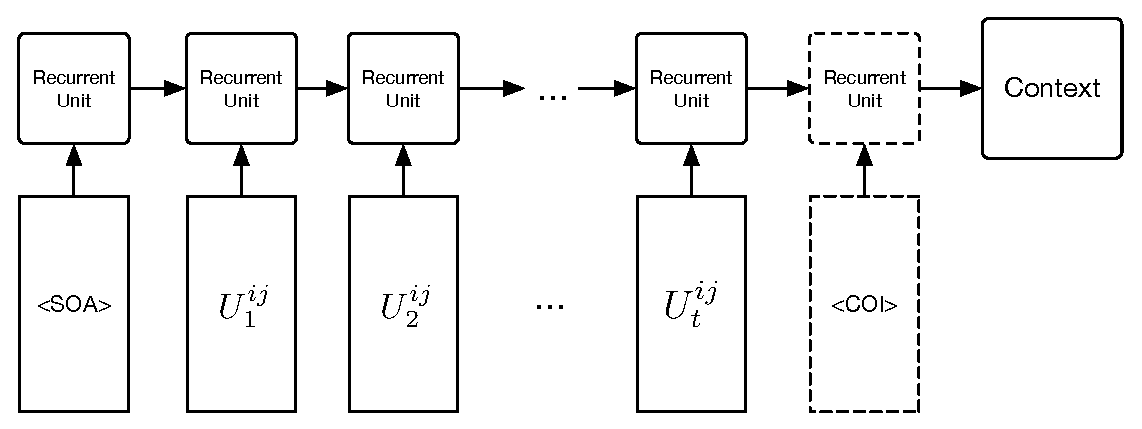
\includegraphics[width=0.7\textwidth]{figures/encoder}
    \caption{Context encoder of Action Path Model. In the encoder, 
    a starting mark ``<SOA>'' is used as a sign of start feeding URLs, 
    and a trigger mark ``<COI>'' as
    a sign to trigger decoder to decodes encoded context tensor.
    The trigger mark is automatically inserted after the $k$-th URL in the end
    of encoder model over time, $k$ is increasing over time.
    In addition, the recurrent unit is not detailly describeed in the figure but afterwards.}
    \label{fig:encoder}
\end{figure}

\subsubsection{Context Decoder}

Context decoder decodes the context tensor produced by encoder. We feed a prediction mark
``<SOP>'' (\emph{Start of Prediction})as a sign to initiate the decoding of encoded context.
In the end of decoder, decoder produces an ending mark ``<EOA>'' (\emph{End of Action}) that
terminates the decoding process.

\begin{figure}[H]
    \centering
    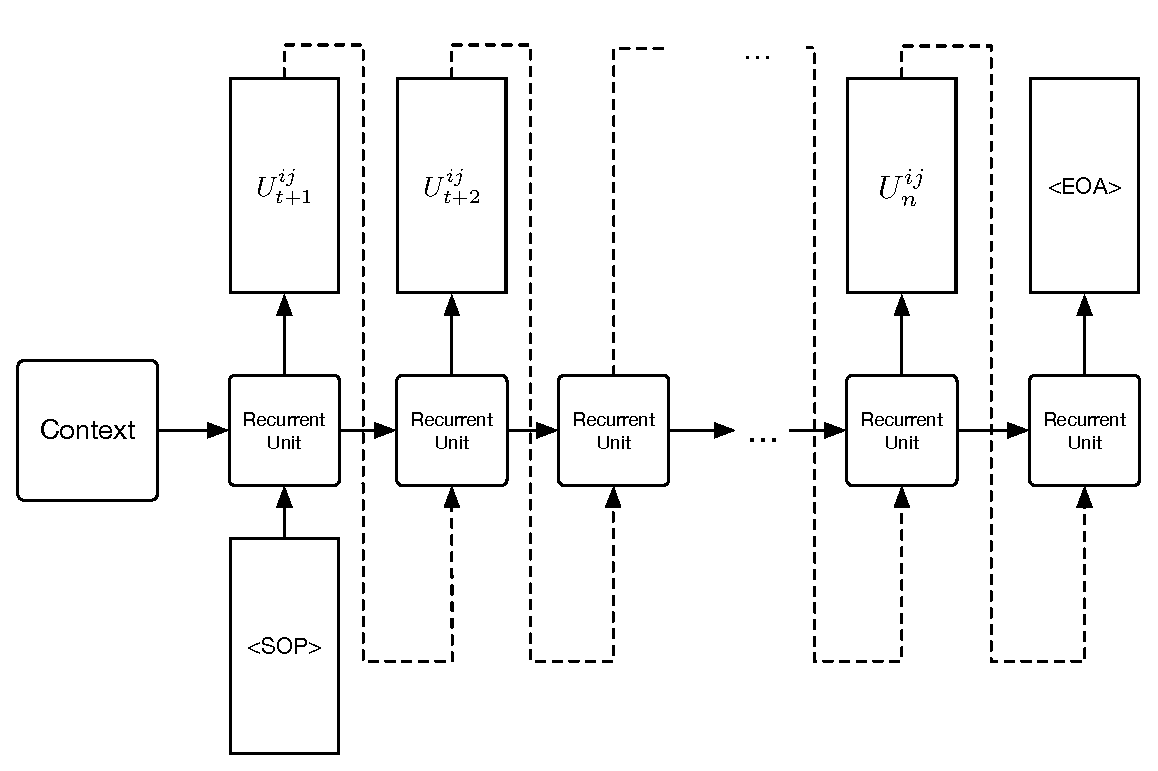
\includegraphics[width=0.7\textwidth]{figures/decoder}
    \caption{Context decoder of Action Path Model. In the decoder, 
    a prediction mark ``<SOP>'' is used to initiate decoding process, 
    and an ending mark ``<EOA>'' as a sign to terminate decode process.
    The output of decoder uses a softmax intermediate operation to magnify and normalize
    the probability of predicted URL embedding.
    In addition, the recurrent unit is not detailly describeed in the figure but afterwards.}
    \label{fig:decoder}
\end{figure}

Note that the decoder model in training phase and prediction phase is different.
In the training phase, teacher forcing strategy \cite{williams1989learning} is used, 
the strategy supplys observed user actions as inputs.
In the testing phase, decoder uses the output from recurrent unit as input, shown through 
dashed lines in Figure \ref{fig:decoder}.

\subsubsection{Recurrent Unit}
\label{sec:recurrent-unit}

The recurrent unit in the Action Path model is not as standard as original 
Long Short-term Memory unit (LSTM)
\cite{hochreiter1997lstm} or 
Gated Recurrent unit (GRU) \cite{DBLP:journals/corr/ChoMGBSB14}.

The original LSTM recurrent unit has a context cell and three regulators: Input gate, 
output gate and forget gate.
The context cell keeps dependencies between inputs of the unit as long term memory. 
Input gate take historical hidden state and current input and controls the input value to
the recurrent unit, output gate responsible for the control of output activations, and
forget gate resets and decides retaining values of the recurrent unit as a short term memory.
Similarly in GRU, it simplyfies the structure of LSTM into a update gate and a reset gate.

In our recurrent unit, when using LSTM as recurrent unit base, we also 
feed time duration $(d^{ij}_1, d^{ij}_2, ..., d^{ij}_n)$
into input gate $I_t$, and others (forget gate $F_t$, output gate $O_t$, 
memory cell $C_t$ and hidden state $h_t$) remains the same:

\begin{align}
\label{eqn:lstm}
\begin{split}
    I_t =& \sigma ( P^{(I)} U^{ij}_t + Q^{(I)} h_{t-1} + \frac{d^{ij}_t}{d^{ij}_t + 1}) ) \\
    F_t =& \sigma ( P^{(F)} U^{ij}_t + Q^{(F)} h_{t-1} + b^{(F)}) \\
    O_t =& \sigma ( P^{(O)} U^{ij}_t + Q^{(O)} h_{t-1} ) \\
    C_t =& F^{(t)} \circ C_{t-1} + I_t \circ \tanh (P^{(C)} U^{ij}_t + Q^{(C)} h_{t-1}) \\
    h_t =& O_t \circ \tanh (C_t)
\end{split}
\end{align}

where $t = 1, 2, ..., n; P^{(I)}, Q^{(I)}, P^{(F)}, Q^{(F)}, P^{(O)}, Q^{(O)}$ are shared weight parameters, 
$b^{(F)}$ is a bias in forget gate $F_t$,
$\circ$ represents element-wise product of two matrices.

When using GRU as recurrent unit base, we feed time duration $(d^{ij}_1, d^{ij}_2, ..., d^{ij}_n)$
in to update gate $Z_t$, and others (reset gate $R_t$, hidden state $h_t$) stay the same:

\begin{align}
\label{eqn:lstm}
\begin{split}
    Z_t =& \sigma ( P^{(Z)} U^{ij}_t + Q^{(Z)} h_{t-1} + \frac{d^{ij}_t}{d^{ij}_t + 1} ) \\
    R_t =& \sigma ( P^{(R)} U^{ij}_t + Q^{(R)} h_{t-1} ) \\
    h_t =& ( 1 - Z_t ) \circ \tanh ( P^{(H)} U^{ij}_t + Q^{(H)} h_{t-1} ) + Z_t \circ h_{t-1}
\end{split}
\end{align}

where $t = 1, 2, ..., n; P^{(Z)}, Q^{(Z)}, P^{(R)}, Q^{(R)}, P^{(H)}, Q^{(H)}$ are shared weight parameters, 
$\circ$ represents element-wise product of two matrices.

\paragraph{Remark 1} The units we described in this section is neither LSTM nor GRU since
the input gate $I_t$ or update gate $Z_t$ introduces time duration $d^{ij}_t$ as input,
which is different than a simple constant bias in the original learnable bias in these gates. 
It is worth mentioning that adding bias to the gates are helpful to 
improve learning performance in LSTM \cite{Jozefowicz:2015:EER:3045118.3045367}, 
we also use the trick in our model as shown in $F_t$ of Equation \ref{eqn:lstm}.

\paragraph{Remark 2} The term $\frac{d^{ij}_t}{d^{ij}_t + 1}$ is a squashing mechanism,
it normalizes $d^{ij}_t$ from $(0, \infty)$ to $(0, 1)$.

\subsubsection{Ending Mark Interpretation}
\label{sec:mark-interpretation}

In context decoder, we mentioned an ending mark ``<EOA>'' that indicates the termination 
decoding process. However, the ending mark is different than other marks, since in practice,
``<EOA>'' is represented in different symbols of behavior-based categorical clickstream, which as a label to
involve classification of user actions.

Assume action paths are labeled by one-hot encoded ending marks 
$\text{EOA}_1, \text{EOA}_2, ..., \text{EOA}_m$ and the last output
of decoder hidden state is $h_n$, we have:

\begin{align}
\label{eqn:lstm}
\begin{split}
    \hat{y} =& \text{argmax} (\text{softmax} (W^{(M)} h_n)) \\
    \hat{y} \in& \{ \text{EOA}_1, \text{EOA}_2, ..., \text{EOA}_m \}
\end{split}
\end{align}

where $W^{(M)}$ is a weight parameter, and $m$ is the number of ending mark categories.

\subsection{Action Path Optimization}

In traditional classification models, the arguments of the maxima (argmax) is used to select
labels with highest probability, scilicet, argmax selects predicted URLs with highest probability
of user action from decoder outputs. However, this method is under the condition of all outputs
are independent in probability, which is not suitable to our senario.

In previous sections, our model feeds an input clickstream $(U^{ij}_1, U^{ij}_2, ..., U^{ij}_t)$,
and produce an output $(o_1, o_2, ..., o_{m})$ that expect close to actual clickstream $(U^{ij}_{t+1}, U^{ij}_{t+2}, ..., U^{ij}_n)$.
Then the probability of expected clickstream is 
a conditional probability under the input clickstream, i.e. we need to solve an optimization problem

\begin{align}
\label{eqn:lstm}
\begin{split}
    & \operatorname*{argmax}_{o} p( o_1, o_2, ..., o_{m} | U^{ij}_1, U^{ij}_2, ..., U^{ij}_t ) \\
   =& \operatorname*{argmax}_{o} \prod_{k=1}^{m} p(o_{k} | U^{ij}_1, ..., U^{ij}_t, o_1, ..., o_{k-1}) \\
   =& \operatorname*{argmax}_{o} \sum_{k=1}^{m} \log p(o_{k} | U^{ij}_1, ..., U^{ij}_t, o_1, ..., o_{k-1})
\end{split}
\end{align}

A heuristic approach can solve the optimization problem efficiently, 
namely beam search \cite{DBLP:journals/corr/abs-1211-3711}. 
In each step of decoder output, we reserve the top-$k$ best combinations of URLs and eliminate the rest of
URLs from evaluation, and finally selects $k$ best clickstreams.
The pseudocode is given that adapts vanilla beam search to URL prediction search in Algorithm \ref{algo:optimize}.

~\\

\begin{algorithm}[H]
\label{algo:optimize}
\SetAlgoLined
\SetKwInOut{Input}{input}\SetKwInOut{Output}{output}
\Input{Decoder outputs $(o_1, o_2, ..., o_{m})$,\\
        Number of candidates $k$}
\Output{k clickstream candidates with highest probability}
\Begin{
    Initialize empty $\text{clickstreams}$ list \\
    \For{$o$ $\in$ $(o_1, o_2, ..., o_{m})$}{
    Initialize empty $candidates$ list \\
    \For{$\text{clickstream}$ $\in$ $\text{clickstreams}$}{
        \For{page $\in$ $o$)}{
            candidates.append([clickstream.append(page), $log(p(\text{clickstream})) + log(p(\text{page}))$]) \\
        }
    }
    ordered = descending order sort candidates by score \\
    clickstreams = ordered[:k]
    }
}
\caption{Output Clickstream Search}
\end{algorithm}

~\\

\paragraph{Remark} The algorithm produces an heuristic output 
with given clickstream context. Combining with \emph{url2vec} model, the prediction
can heuristically optimize the click path of a specific user since the embeddings are trained 
over all possible action path. For instance, a distraction advertisement page will not appear
after optimization because the embedding of advertisement page is far from a desired page
if embeddings are learned correctly.

% This chapter proposed several models that characterized a method to modeling user actions
% on the Web.

\cleardoublepage